\begin{figure}[h][p]
    \centering
    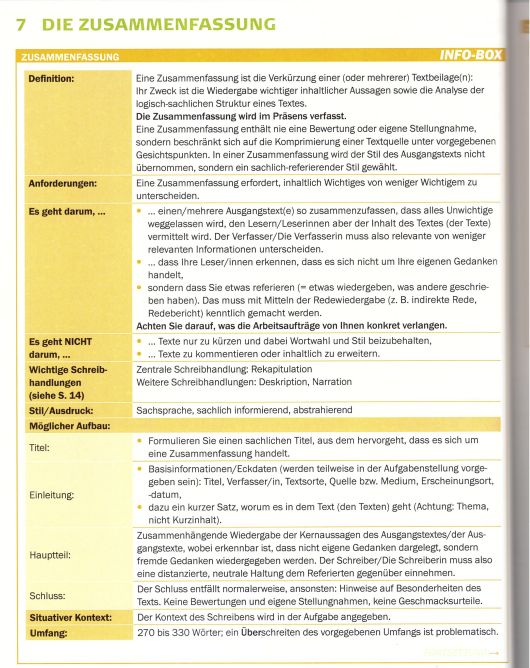
\includegraphics[scale=0.8]{./pics/Screenshot from 2023-02-06 12-32-33.png}
    \caption{Zusammenfassung: Definition + Aufbau}
    \label{fig:impl:Zusammenfassung1}
\end{figure}
\begin{figure}[h]
    \centering
    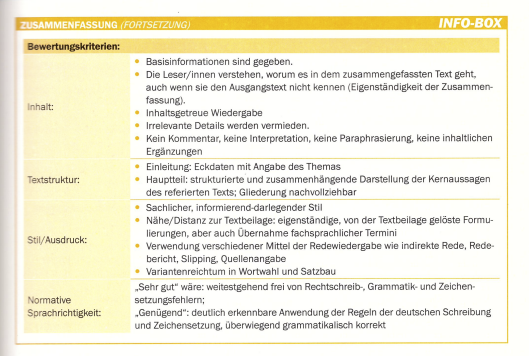
\includegraphics[scale=0.8]{./pics/Screenshot from 2023-02-06 12-33-05.png}
    \caption{Zusammenfassung: Verfassen}
    \label{fig:impl:Zusammenfassung2}
\end{figure}
\begin{figure}[h]
    \centering
    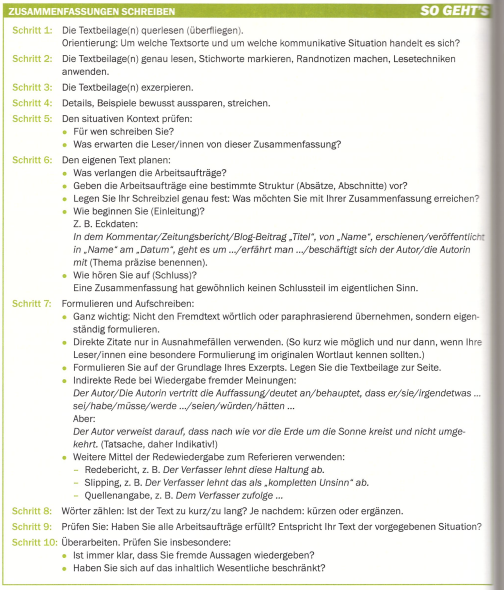
\includegraphics[scale=0.8]{./pics/Screenshot from 2023-02-06 12-33-47.png}
    \caption{Zusammenfassung: Fortsetzung}
    \label{fig:impl:Zusammenfassung3}
\end{figure}
  

\section{Mustertext}


\section{Eigener Text}

Lesen Sie den Zeitungsbericht „Die junge Generation ist benachteiligt“, der von Wolfgang Böhm verfasst wurde und in Die Presse am 13. November 2016 veröffentlicht wurde. Schreiben Sie nun eine Zusammenfassung und bearbeiten Sie folgende Arbeitsaufträge: Geben Sie die wichtigsten Inhalte hinsichtlich Jugendarbeitslosigkeit wieder. Beschreiben Sie die Vorzüge, die sich für die ältere Generation ergeben. Erschließen Sie die notwendigen Schritte, um einen sozialen Kollaps zu vermeiden.  

Schreiben Sie zwischen 270 und 330 Wörter. Markieren Sie Absätze mittels Leerzeilen 

\subsubsection{Die junge Generation ist benachteiligt!}
Der Artikel „Die junge Generation ist benachteiligt“ von Wolfgang Böhm (Die Presse), welcher am 13.11.2016 erschienen ist, handelt von den Auswirkungen der Finanzkriese 2007. Vor allem der große Unterschied zwischen den Jugendlichen und Menschen über 65 wurde stark herausgehoben.  

Konkret geht es darum, dass vor allem die Älteren es geschafft haben, eine gewisse Sicherheit zu wahren, während bei den Jungen die Unsicherheit und die Angst der Zukunft wuchs. In Zahlen ausgedrückt heißt es, dass während der Krise die Zahl der Arbeitslosen Jugendlichen bei 26.4 \% lag, sie danach bei 26.9\%. Im Vergleich, bei den über 65-Jährigen schrumpfte der Anteil von 23.3\% auf 17.4 Prozent. Auch in den Zahlen der schwerwiegenden Entbehrungen spiegelt sich die Situation wider. Während 9.5\% der Jugendlichen in Europa ihre Grundbedürfnisse nicht decken können, sind es bei den Älteren lediglich 5.5 Prozent. Auslöser dafür war während der Krise die Tatsache, dass sich die Gehälter und Pensionen älterer Arbeitnehmer kaum gekürzt wurden, jedoch das Einkommen der Jungen stark zurück ging.   

Laut der Studie ist die soziale der Jugend heute in keinem einzigen EU-Landbesser als im Jahr 2008. Österreich ist keine Ausnahme. Waren 2007 hier 16,7 Prozent der Kinder und Jugendlichen (bis zu 18 Jahren) von Armut oder sozialer Exklusion bedroht, so sind es heute 18,3 Prozent. Bei der Generation der über 65-Jährigen ging dieses Risiko von 21,2 auf 14 Prozent zurück. Auch besonders bemerkenswert ist das deutliche Nord-Süd-Gefälle. Jugendliche aus Nordeuropa haben noch eher Chancen auf einen Arbeitsplatz und ein geringeres Armutsrisiko als jene aus Südeuropa.  

Am Ende des Artikels wird zu Arbeitsmarkt und Bildungspolitik Reformen aufgerufen, da sich die Lage der Jugendlichen zu verschlechtern scheint. Kinder aus ärmeren Familien haben deutlich geringere Chancen, ein höheres Bildungsniveau zu erreichen als Kinder wohlhabender Eltern. Länder wie Finnland oder Estland seien hier vorbildlich. 
\section{Formulierungshilfen}

Einleitung:
enthält: Autor, Titel, Textsorte, Erscheinungsjahr/-datum, ggf. Erscheinungsort, kurze Benennung des Themas 
\begin{compactitem}
    \item Das/ Der /Die (Textsorte) „(Titel)“ von (Autor) aus dem Jahr .... beschreibt .../handelt von.../ thematisiert...  
    \item In dem (Zeitungsartikel) „(Titel)“ von (Autor) erschienen in (Erscheinungsort/ Herausgeber) am (Erscheinungsdatum) geht es um... 
\end{compactitem}
Hauptteil: 
\begin{compactitem}
    \item  Zu Beginn berichtet der Autor.../ spielt die Handlung... 
    \item  Anfangs wird festgestellt... / darauf hingewiesen, dass...
    \item  Eingangs .../ Zunächst.../ Bevor...
    \item Die Kurzgeschichte/ Der Roman/ Das Drama beginnt damit, dass... 
    \item Später geht der Autor darauf ein, dass... 
    \item  Im Folgenden... / Es folgt...
    \item Danach... / Später wird klar, dass...
    \item Im Verlauf der Geschichte/ des Berichtes/ des Kommentars etc. wird deutlich, dass...
    \item Plötzlich greift... in das Geschehen ein und.../ indem...
    \item  Die Situation beginnt sich zu verändern, als .../ nachdem... 
    \item Die Geschichte endet mit...
    \item Die Situation wird aufgelöst durch.../, indem.../ als..
    \item Schließlich .../ Am Ende.../ Zum Schluss... 
    \item Abschließend betont der Autor (nochmals), dass 
\end{compactitem}

Schluss:
\begin{compactitem}
    \item  Auf mich wirkt der Text... 
    \item  Zusammenfassend ist also pointiert festzuhalten, dass… 
    \item Letztlich bleibt anzumerken... 
    \item Als einzig logisches Fazit lässt sich also festhalten, dass...
    \item Abschließend ist daher anzunehmen, dass... 
    \item m Vergleich zu... ist es in diesem Text/ diesem Autor (nicht) gelungen... 
\end{compactitem}